\documentclass{article} % For LaTeX2e
\usepackage{nips15submit_e,times}
\usepackage{hyperref}
\usepackage{url}
\usepackage{graphicx}
\usepackage{subcaption}
\usepackage{amsthm}
\usepackage{amssymb}
\usepackage{algorithm}
\usepackage[noend]{algpseudocode}
\usepackage{centernot}

\newcommand{\Expect}{{\rm I\kern-.3em E}}
\algdef{SE}[DOWHILE]{Do}{doWhile}{\algorithmicdo}[1]{\algorithmicwhile\ #1}

\usepackage{mathtools}

\DeclarePairedDelimiterX{\infdivx}[2]{(}{)}{%
  #1\;\delimsize\|\;#2%
}
\newcommand{\infdiv}{D\infdivx}
\DeclarePairedDelimiter{\norm}{\lVert}{\rVert}

\theoremstyle{definition}
\newtheorem{definition}{Definition}[section]
\newtheorem{theorem}{Theorem}[section]
\newtheorem{corollary}{Corollary}[theorem]
\newtheorem{lemma}[theorem]{Lemma}
\newtheorem{assumption}{Assumption}
\newtheorem{prop}{Proposition}
%\documentstyle[nips14submit_09,times,art10]{article} % For LaTeX 2.09
\title{}
\author{}
\newcommand{\fix}{\marginpar{FIX}}
\newcommand{\new}{\marginpar{NEW}}
\nipsfinalcopy % Uncomment for camera-ready version
\begin{document}

\maketitle

\begin{abstract}
We seek to contribute:\\
1) A clear understanding of partial observability.\\
2) A measure of the degree to which a domain is partially observable.\\
3) A way to quantify the deficiency of a given state representation.\\
\end{abstract}

%% \section{Definitions}
%% The following definitions assume a fixed state representation. If we
%% have the ability to manipulate the state representation, the same
%% stochastic process can be Markov or non-Markov.


%% \begin{definition}[k-order Markov Chain]
%% A Markov chain of order $k$ has the property that:
%% \[
%% P(s_{n+1} | s_{n}, s_{n-1}, \dots, s_{1}) = P(s_{n+1} | s_{n}, \dots, s_{n-(k-1)})
%% \]
%% The future state $s_{n+1}$ depends on the past $k$ states. Remembering
%% $k$ states restores the Markov property and a larger memory grants no
%% further predictive power.
%% \end{definition}

\section{Introduction}
The relationship between state, observation, reward, and task, is
nuanced and deserves careful attention. Much of the discussion below
stems from the careful analysis of state and observability presented
in Andrew McCallum's thesis \cite{McCallum96}.

At a high level, reinforcement learning begins with an idea of a task
that a learning agent should perform. Two example tasks which we will
revisit are Texas Hold'em and autonomous driving. In the first task,
one might desire the agent to learn to play the card game Texas
Hold'em, and be capable of competing against other players. In
autonomous driving the agent must learn how to safely control the
vehicle in the presence of other drivers and navigate to a
destination. Reinforcement learning requires more than general concept
of desired functionality. Formally, we define a reinforcement learning
task as follows:

\begin{definition}[Reinforcement Learning Task]
\label{def:markov}
A reinforcement learning task $\mathcal{Z} = (\Omega, A, R, \gamma ||
S, \mathcal{O}, r, \mathcal{P})$ is defined by an observation space
$\Omega$, action space $A$, reward space $R$, and discount factor
$\gamma \in [0,1]$. All of these components are known by the agent
apriori. Additionally, every task has some components that are hidden
from the agent (denoted by everything following $||$). In particular
there is a task-relevant-state-space $S$ (formalized in Definition
\ref{def:taskRelState}), an observation distribution $\mathcal{O}: S
\times \Omega \rightarrow \mathbb{R}$, a reward function $r : S \times
A \rightarrow \mathbb{R}$, and a transition probability distribution
$P : S \times A \times S \rightarrow \mathbb{R}$.

Specifically, the agent's interaction with the environment is broken
down into discrete timesteps. Let $\pi$ denote the agent's policy $\pi
: \Omega \times A \rightarrow [0,1]$. At each timestep, the agent receives
some observations $o \in \Omega$ from the environment, selects an
action $a \in A$ to perform according to $\pi(a | o)$, and receives a
reward $r \in R$. The state of the environment $s \in S$ transitions
according to the environment's dynamics: $s' \sim P(s,a)$ as does the
agent's observation $o' \sim \mathcal{O}(s')$. This pattern of
interaction continues until the episode ends.
\end{definition}

Since observations may encode incomplete information about the state
of the world, it can be beneficial for an agent to retain a memory of
over past observations. We denote a memory-based policy using the
following notation: $\pi_n : \Omega^3 \times A \rightarrow
[0,1]$. Specifically, the memory-based policy considers the latest $n$
observations $\pi_n(a|o_t, o_{t-1}, \dots, o_{t-(n-1)})$. $\pi_\infty$
is a policy that retains memory of the full observation sequence.

The expected return of a policy is denoted as follows: $\eta(\pi_1) =
\Expect_{o_0, a_0, \dots} \Big [ \sum_{t=0}^\infty \gamma^t r(s_t)
  \Big ]$ where $a_t \sim \pi_1(a_t|o_t)$. A reinforcement learning
task induces at least one optimal policy $\pi^*_\infty$, such that
$\eta(\pi^*_\infty) \ge \eta(\pi_n)$ for all possible $\pi_n$. More
generally, it's possible to consider optimal policies over any length
of memory, for which the following inequality holds:
$\eta(\pi^*_\infty) \ge \dots \ge \eta(\pi^*_2) \ge
\eta(\pi^*_1)$. Building on the concept of optimality, we define two
properties of observation spaces:

\begin{definition}[$n$-Policy-Markov]
Let us consider the performance of different memory-based optimal
policies in some task $\mathcal{Z}$. The observation space of
$\mathcal{Z}$ is n-Policy-Markov if $\eta(\pi^*_n) =
\eta(\pi^*_\infty)$. In other words, maintaining a memory of the last
$n$ observations is sufficient to perform as well as a policy that
remembers a complete history of observations.

$n$-Policy-Markov is similar to $k$-order Markov property. However,
while the Markov property is concerned with probability distributions
over next states, $n$-Policy-Markov focuses on returns of optimal
policies. While the ability to predict future state is useful, the
more practical concern is that of maximizing return. Thus the
$n$-Policy-Markov definition is more useful than the standard
$k$-order Markov property.
\end{definition}

Another useful definition allows two observation spaces to be compared
in terms of optimal policies:

\begin{definition}[Optimally-Equivalent]
\label{def:opt-equiv}
Consider a task $\mathcal{Z}$ with observation space $\Omega$ and a
related task $\mathring{\mathcal{Z}}$ that is identical except its
observation space $\mathring{\Omega}$ and observation function
$\mathring{\mathcal{O}}$. Such a situation could arise when testing
new sensors for an autonomous vehicle - each new sensor alters the
observation space and may affect the achievable return of an optimal
policy.

The observation space $\Omega$ is said to be
\textit{optimally-equivalent} to $\mathring{\Omega}$ if the return of
a non-memory-based optimal policy over $\Omega$ equals the return of a
non-memory-based optimal policy over $\mathring{\Omega}$:
\[
\eta \big(\pi^*_1(\cdot|o \in \Omega) \big) = \eta \big(\pi^*_1(\cdot|o \in \mathring{\Omega}) \big)
\]
Notationally, we denote optimal equivalence using the following
shorthand: $\Omega \overset{*}{\equiv} \mathring{\Omega}$. We will
also consider optimal-equivalence between state and observation
spaces: $\Omega \overset{*}{\equiv} S$. Such a situation would imply
that maintaining a memory over observations is unnecessary.
\end{definition}

To understand the purpose of these definitions, let us consider the
omnipotent agent. This imaginary agent has access to the true state of
the entire universe down to the locations of every particle in every
galaxy (and enough computation to learn from this representation). As
a result, the omnipotent agent, when presented with a task
$\mathcal{Z}$, will always ignore the task-defined observations,
instead preferring to rely on its own observations. Formally, it is
operating in a different task $\mathring{\mathcal{Z}}$, where the
task-defined observations have been replaced with the agent's own
observations $\mathring{\mathcal{S}}$. This new state space includes
an optimal policy $\mathring{\pi}^*: \mathring{\mathcal{S}}
\rightarrow \mathcal{A}$ that is at least as good as the optimal
policy in the observation space:
$\mathring{\mathcal{J}}^{\mathring{\pi}^*} \ge
\mathcal{J}^{\pi^*}$. The original observation space of $\mathcal{Z}$
may be noisy or lack relevant information for performing the task. The
omnipotent agent's state representation suffers neither of these
flaws.

Setting observations aside for a moment we briefly focus on state
representations. It's typically not necessary to observe the entire
universe in order to learn an optimal policy for a task. We posit that
for any task $\mathcal{Z}$ there is a more compact state
representation $\mathcal{S}_\mathcal{Z}$ that is optimally-equivalent
to $\mathring{\mathcal{S}}$, the omnipotent
observation. $\mathcal{O}_\mathcal{Z}$ captures the
\textit{task-relevant-state} and ignores information that is
irrelevant to the task at hand. For task $\mathcal{Z}$, the set of
optimal policies defined over $\mathcal{S}_\mathcal{Z}$ is equivalent
to the set of optimal policies over $\mathring{\mathcal{S}}$. In Texas
Hold'em, the task-relevant-state includes knowledge of the cards in
other players' hands, knowledge of the order of cards in the deck, and
emotional states of the other players, but does not include
inconsequential information such as the temperature on top of Mount
Everest. While the notion of an omnipotent agent is purely
theoretical, task-relevant-state spaces are well defined for
single-player games like Solitaire, in which the order of the cards in
the deck as well as the face-up cards provide a task-relevant-state.

\begin{definition}[Task-Relevant-State]
\label{def:taskRelState}
A task-relevant-state representation $\mathcal{S}_\mathcal{Z}$ is a
more compact representation of universe-state $\mathring{\mathcal{S}}$
that is both Policy-Markov and optimally-equivalent to
$\mathring{\mathcal{S}}$ for the task
$\mathcal{Z}$. Task-relevant-state is exactly the state representation
desired in a Markov Decision Process as it allows a reactive,
memory-free agent to learn an optimal policy that performs as well as
if the agent was omnipotent. However, many tasks lack a well defined
or computable task-relevant-state. Regardless, the notion of
task-relevant-state will be useful in subsequent analysis.
\end{definition}

The complexity and fun of many tasks stems from hidden state. For
example, Texas Hold'em is intended to be played with partial
information. Every task must define an observation space - in the case
of Texas Hold'em, a reasonable observation space is the player's cards
and community cards. In autonomous driving, the observations may be
perceptions from the laser range-finders, cameras, and other sensory
equipment. In the best case, the observation space may provide a
task-relevant-state. In general though, the observation space is
likely to be noisy or lack task-relevant information. A contribution
of this paper is a way to quantify the degree to which an observation
space falls short of being a task-relevant-state-space. At a high
level, there are two types of loss that may be experienced:

In the case of \textit{irreversible-information-loss}, observations
may irreversibly lose important state information: for example, the
Texas Hold'em agent can't perceive the community cards, or the
autonomous vehicle's range-finder is broken. In both cases, even
maintaining a full memory over past observations will not help recover
the missing information, which is irreversibly lost.

In the more benign case of \textit{memory-reversible-loss}, the
observation space is non-Policy-Markov, meaning that a memory of past
observations yields better optimal policies. In Texas Hold'em, it
could be useful to remember that another player tends to bluff often
and use this fact to call her raise. Memory reversible loss refers to
any information that can be inferred by maintaining a history of
obseravtions.

In general, an observation space may feature a mix of irreversible
information loss and memory reversible loss. Historically, this
information loss has been referred to as \textit{Partial
  Observability}. We now visit the concept of partial observability in
greater detail.

\section{Partial Observability}
In the context of reinforcement learning, partial observability
describes a task in which the task-defined observations fall short of
being task-relevant-states. This problem is also known as
\textit{incomplete perception}, \textit{perceptual aliasing}, or
simply \textit{hidden state}.

There are two causes of partial observability. One cause of is
perceptual aliasing, in which multiple states all map to the same
observation. Another cause is noisy perceptions, in which a state is
observed differently each time it is revisited. Figure
\ref{fig:functions} illustrates these cases.

\begin{figure}[htp]
\centering
\begin{subfigure}{.3\textwidth}
  \centering
  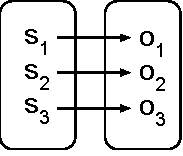
\includegraphics[width=.6\linewidth]{figures/bijection}
  \caption{Fully Observed}
  \label{fig:bijection}
\end{subfigure}
\begin{subfigure}{.3\textwidth}
  \centering
  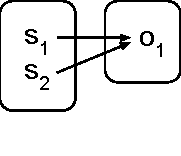
\includegraphics[width=.6\linewidth]{figures/state-aliasing}
  \caption{State Aliasing}
  \label{fig:state-aliasing}
\end{subfigure}
\begin{subfigure}{.3\textwidth}
  \centering
  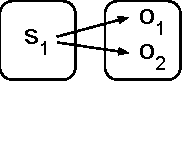
\includegraphics[width=.6\linewidth]{figures/noisy-perception}
  \caption{Noisy Perceptions}
  \label{fig:noisy-perception}
\end{subfigure}
\caption{A fully observed environment features an injective mapping
  from task-relevant-states to observations. Partial observability
  indicates the degree to which this injection is invalid. Two sources
  of partial observability are state aliasing: the degree to which the
  observation function is non-injective, and noisy perceptions: the
  degree to which the observation function is not a valid function.}
\label{fig:functions}
\end{figure}

\begin{definition}[Partial-Observability]
\label{def:PO}
A task is fully observed if and only if its observation space is
optimally-equivalent to the task-relevant-state. Otherwise, it is
partially observed.
\end{definition}

To better understand this definition, we consider several cases: If
the observation space is the task-relevent-state, then the optimal
policies in both representations will be the same and the task may be
said to be fully observed. Furthermore, any representation that yields
equivalent optimal policies is sufficient for full observability. It's
not necessary to have direct access to the task-relevant-state
representation so long as the optimal policies over the available
observations perform equivalently well.

\subsection{Tests for Partial Observability}
While the definition above helps to understand the concept of partial
observability, it does not provide a way to directly test whether a
given task is partially observed. This section presents three tests
for partial observability that follow directly from the definition
above:

\begin{enumerate}
\item With access to a task-relevant-state: A task is fully observable
  if and only if the mapping from task-relevant-states to observations
  is one-to-one (injective). Otherwise it is partially observable. The
  possible deviations from an injective mapping are shown in Figure
  \ref{fig:noisy-perception}.
\item With access to an oracle: A task is partially observable if the
  optimal policy $\pi^*$ learned over the observation space performs
  worse than the oracle. For example, in autonomous driving if an
  optimal policy over a given observation space does not perform as
  well as a human driver, it may be concluded that the observation
  space is partially observerable (assuming equivalent reward
  functions for the human driver and optimal policy).
\item With access to neither: A task is partially observable if it is
  non-Policy-Markov. This is to say, if an optimal policy that has
  access to a history of observations performs better than an optimal
  policy without access to an observation history. This is exactly the
  case of partial observability stemming from \textit{reversible
    information loss}. Note, the other direction does not hold: if the
  memory-based optimal policy does not outperform the memory-free
  optimal policy, it is still possible that the task is partially
  observed. Such is the case with
  \textit{irreversible-information-loss}.
\end{enumerate}

\begin{prop} Markov property is orthogonal to Partial-Observability\\
We consider two cases that demonstrate that the Markov property is not
sufficient to determine if a task is partially observed.
\begin{enumerate}
\item Non-Markov $\centernot\implies$ Partially Observed: Consider a
  representation that consists of the task-relevant-state plus an
  extra feature that encodes a periodic function (e.g. sin,
  cosine). This task is non-Markov because predicting the next value
  of a periodic function requires more than an observation of the
  current value. However, the task is also fully observed, because its
  representation is optimally equivalent to the task-relevant-state,
  e.g. the same optimal policies exist simply by ignoring the periodic
  feature.
\item Markov $\centernot\implies$ Fully Observed: Consider a representation
  that consists of a single unchanging feature (perhaps as a result of
  extreme irreversible information loss). This representation is
  Markov, because it requires no history to predict the next value of
  this feature. However, this degenerate representation is not
  optimally-equivalent to the task-relevant-state, and thus the task
  is not fully observed.
\end{enumerate}
\end{prop}

While there is some value in determining whether or not a task is
partially observable, most real world tasks are clearly partially
observable and the quantity of interest is \textit{how} partially
observed they are, and perhaps how to augment the observation space
towards the task-relevant-state. The next section presents one way to
quantify the degree of partial observability in a task.

\section{An Information-Theoretic View of Partial Observability}
We first review some fundamental concepts of information theory:

\begin{definition}[Entropy]
\label{def:entropy}
The entropy of a discrete random variable $X$ with alphabet $\mathcal{X}$ is
defined by:
\[
H(X) = -\sum_{x\in \mathcal{X}} p(x) \log p(x)
\]
\end{definition}

Entropy provides a way of understanding how uncertain an event is of
occurring, alternatively how many bits of information is required to
transmit the outcome of an event. We aim to compute entropy over
distributions of states. A highly entropic state distribution would be
one in which each visited state is unique.

\begin{definition}[Mutual Information]
The mutual information between two random variables $I(X;Y)$ is the
reduction of uncertainty of $X$ due to knowledge of $Y$:
\[
I(X;Y) = \sum_{x,y} p(x,y) \log \frac{p(x|y)}{p(x)} = H(X) - H(X|Y)
\]
\end{definition}

One way to understand the partial observability of a task is to
quantify the amount of information the observations provide about the
task-relevant-states. Let us assume we have access to the true
task-relevant-state which generates each observation. Let $S$ be a
random variable over the domain of all possible states, and $O$ be a
random variable over all possible observations. The mutual information
$I(S;O)$ computes the reduction in uncertainty of the true environment
states $S$ resulting from knowledge of the observations $O$:

\[
I(S;O) = \sum_{s,o \in S \times O} p(s,o) \log \frac{p(s|o)}{p(s)} = H(S) - H(S|O)
\]

If the mapping from task-relevant-states to observations is
one-to-one, the mutual information $I(S;O)$ will equal $H(S)$, and the
agent's interaction with the environment is said to be fully observed.

\section{Using a History of Observations}
A natural technique to deal with partial observability is to augment
the agent's state representation to include a history of
observations. This strategy helps to address state aliasing by using
the observation history to disambiguate aliased states. In the case of
noisy observations, a history could be used to counteract noise, for
example by smoothing recent observations. However, the size of the
state space grows exponentially as a function of history length, so in
practice it is rarely feasible to maintain extensive history.

\begin{definition}[k-th Order Mutual Information]
Let $\textbf{O}^k$ be a random variable over the domain of all
k-length observation sequences $\textbf{o}^k = (o_t, o_{t-1}, \dots,
o_{t-(k-1)})$. We define the $k$-th order mutual information between
$k$-length observation histories and true states as follows:

\[
I(S;\textbf{O}^k) = \sum_{s,\textbf{o}^k \in S \times \textbf{O}^k} p(s_t,\textbf{o}^k) \log \frac{p(s|\textbf{o}^k)}{p(s)}
\]
\end{definition}

The growth of $I(S;\textbf{O}^k)$ as a function of $k$ reveals the
predictive power gained by leveraging additional history. Even
maintaining a full history cannot guarantee full observability in all
cases: in an extreme case where all states are mapped to the state
observation, even a full history is no help in predicting the next
state.

\section{Entropy of Atari Games}
The state of an Atari game is fully specified by the 1024-bits of
console RAM. The Atari environment defines an observation function
$O(o|s)$ that maps RAM states to observed screens. This true state is
invisible to humans, who instead see the $160 \times 210 \times 3$
dimensional screen. Fortunately, the Arcade Learning Environment
provides access to both the RAM states and observed Atari screens.

A single Atari game screen often does not contain enough information
to disambiguate important aspects of state. Two examples: in the game
of Breakout, a single frame is sufficient to locate the position, but
not velocity, of the ball, which is necessary in order to correctly
position the paddle. Similarly, the player and opponent bullets in
Space Invaders look identical, so the only way to tell if a bullet is
approaching your ship or leaving it is to look at more than one
screen.

RAM states contain sufficient information to entirely restore the
state of the Atari game. However, RAM states are not exactly
task-relevant-states because they contain information that is
irrelevant to \textit{playing} the game. For example, many games such
as Seaquest feature animated backgrounds that are irrelevant to actual
gameplay, but require RAM to encode.

\subsection{Atari RAM Entropy}
We expect the RAM-entropy of will differ on a game-to-game
basis. There are several problems applying the standard definition of
entropy (Def \ref{def:entropy}) to Atari RAM-states:

\subsection{Stationary State Distribution}
In order to compute entropy, a distribution over RAM-states is
required. Atari does not provide access to the true distribution over
RAM-states, but instead allows sampling from this distribution in the
form of playing the game and recording the encountered
RAM-states. From any set of recorded RAM-states it is possible to
construct a distribution, but the constructed distribution may not
resemble the game's true distribution over RAM-states. In particular,
two questions arise: 1) What policy should be used to sample
RAM-states and 2) How many samples are necessary to ensure the
constructed distribution closely resembles the true distribution?
Before addressing these questions, let us define several
preliminaries:

\begin{definition}[Ergodic MDP]
An MDP $\mathcal{M}$ is ergodic if the Markov chain induced by any
policy is ergodic. An ergodic MDP is an MDP where every state can be
accessed in a finite number of steps from any other state.
\end{definition}

\begin{definition}[Episodic MDP]
An episodic MDP is an MDP with a terminal state that is accessible
from any state.
\end{definition}

\begin{definition}[Stationary State Distribution of Ergodic MDP]
\label{def:ssd}
An ergodic MDP has a stationary distribution $d^{\pi}(s)$ with the property:
\[
d^\pi(s) = \sum_{s' \in S} d^\pi(s')\mathcal{P}_{s',s}
\]
\end{definition}

Atari games are episodic MDPs with deterministic transitions. Formally,
episodic MDPs can never be ergodic since terminal states never
transition to any other state. However, it is possible to convert an
episodic MDP into an ergodic MDP by constructing an equivalent MDP
with each terminal state having a single action that transitions the
agent to the starting state.\footnote{The transition from the terminal to
starting state should have a discount factor of zero in order to
maintain equivalence of optimal values \cite{VanHasselt11}.}

Thus, playing multiple episodes of a given game under a fixed policy
$\pi$ is sufficient to define an ergodic MDP, and by definition
\ref{def:ssd}, for any fixed policy $\pi$, the Markov chain induced by
$\pi$ should have a stationary state distribution $d^\pi_\infty$. The
\textit{mixing time} of the Markov chain is the minimum amount of time
$t$ needed to ensure that $d^\pi_t$, the state distribution
constructed after $t$-steps, is epsilon close to the true stationary
state distribution $d^\pi_\infty$ (e.g. the distribution that would be
constructed after an infinite number of samples).

\begin{definition}[Mixing Time]
\label{def:ssd}
The mixing time $t_{\mathrm{mix}}(\epsilon)$ of an ergodic MDP is given by:
\begin{align*}
t_{\mathrm{mix}}(\epsilon) & = \min_t \norm{d^\pi_t - d^\pi_\infty}_{TV} \le \epsilon \\
& = \tfrac{1}{2}\sum_{s \in S} |d^\pi_t(s) - d^\pi_\infty(s) | \le \epsilon
\end{align*}
where $\norm{\cdot}_{TV}$ indicates the total variation distance.
\end{definition}

In general, it's hard to estimate mixing time...

In general, the distribution over visited states is a function of the
policy.



\begin{algorithm}
\caption{Dataset Collection}
\label{ram-ent}
\begin{algorithmic}
\State Given: Policy $\pi$, Error Bound $\epsilon$
\State $\mathcal{D} \gets \{\emptyset\}$ \Comment{$\mathcal{D}$ is the collection of all trajectories}
\Do
\State $\mathcal{D} \gets \mathcal{D}\ \cup \ $PlayEpisode$(\pi)$
\State $d^\pi_t \gets \ $ComputeStationaryStateDistribution($\mathcal{D}$)
\State $t\gets t+1$
\doWhile{$\norm{d^\pi_t - d^\pi_\infty}_{TV} > \epsilon$} \Comment{Wait until the state distribution converges}
\State \Return $d^\pi_t$
\end{algorithmic}
\end{algorithm}

\begin{definition}[Observability]
Assuming access to the true state distribution $S$ of an environment
as well as the observation distribution $O$, the observability
$\mathcal{O}$ of the environment is given by conditional entropy of
the true states given the observations, divided by the entropy of the
states.
\[
\mathcal{O} = 1 - \frac{H(S|O)}{H(S)}
\]
The observability quantifies how much information the observations
possess about the true environment state. Observability is always
between zero and one: an observability of zero indicates the
observations are no help in understanding the environment's state. An
observability of one implies the observations fully determine the true
state. Observability measure the degree of bijectivity in an
environment's mapping from states to observations.
\end{definition}


\section{Half Baked Ideas}
The following sections contain intuitions that may have some promise
but are poorly grounded.

\section{Sub-optimality induced by partial observability}
Partial observability causes agents to learn sub-optimal policies. The
degree of partial observability inherent in an environment bounds the
performance of an optimal policy learned over observations $\pi_O^*$
compared to the optimal policy learned over true states $\pi_S^*$:
\[
\textrm{sub-optimality} \propto \sum_{s\in S} D_{KL}\big(\pi_O^*(O(s))\ ||\ \pi_S^*(s)\big)
\]

\bibliographystyle{unsrt}
\bibliography{partialobs}
\end{document}
